%\section{OpenBTS}
\utsection{OpenBTS}{Max Eschenbacher}
\textbf{OpenBTS (Open Base Transceiver Station)} ist eine freie Unix-Applikation die in C++ entwickelt wurde. Mit Hilfe eines Software Radios und der entsprechenden Hardware, kann OpenBTS die GSM Luftschnittstelle \textit{Um} simulieren. In Verbindung mit einer Private Branch Exchange (PBX) können die Mobilfunkteilnehmer untereinander, sowie, je nach Anbindung, mit VoIP- bzw. Festnetzteilnehmern telefonieren.

\subsection{Aufbau und Zusammenspiel}
\subsubsection{Komponenten}
Ein funktionsfähiges OpenBTS System besteht aus folgenden Komponenten:

\begin{itemize}
\item \textbf{OpenBTS}\\
Die eigentliche Kernsoftware, welche (fast) den gesamten GSM-Stack oberhalb des Radios realisiert.
\end{itemize}
\begin{itemize}
\item \textbf{Transceiver}\\
Kombination aus Radio-Hardware (USRP1) und der ansprechenden Software (GNUradio). Dadurch wird der gesamte Physical Layer der GSM \textit{Um} Luftschnittstelle realisiert. Die eingesetzte Universal Software Radio Peripheral (USRP) ist von der Firma Ettus Research (siehe Abbildung \ref{fig:usrp1}) und wird über einen FA-Synthesizer (siehe Abbildung \ref{fig:fasyn}) mit 52MHz betrieben.
\begin{figure}[htbp]
  \centering
  \begin{minipage}[b]{6cm}
    \centering
    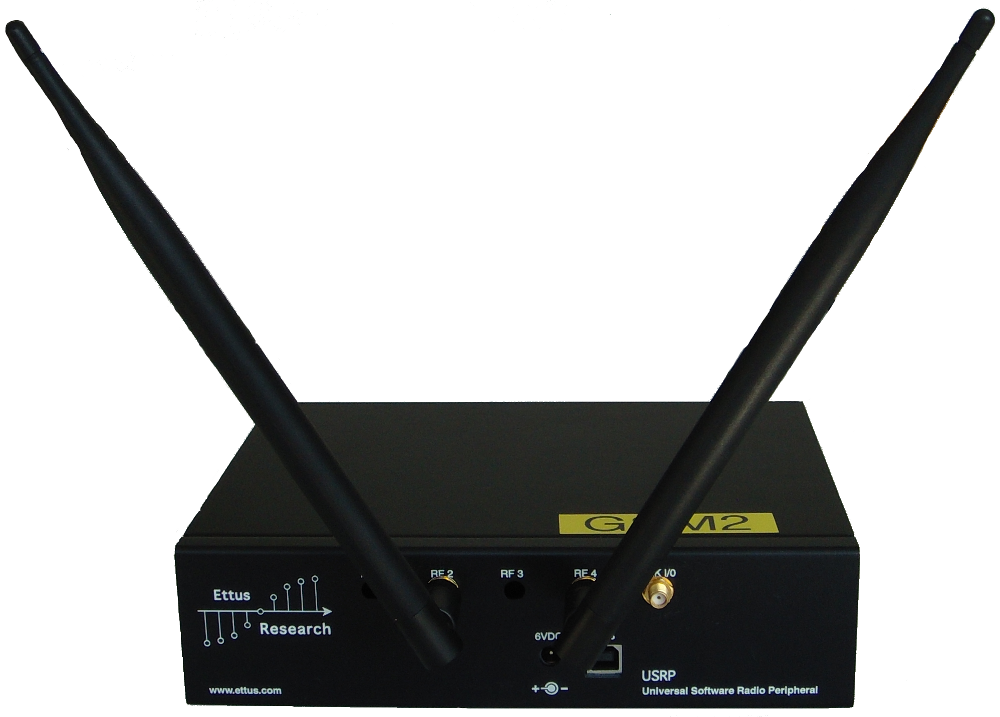
\includegraphics[width=1.00\textwidth]{img/usrp1.png}
    \caption{GSM-Radio USRP1}
	\label{fig:usrp1}
  \end{minipage}
  \begin{minipage}[b]{2cm}
  \end{minipage}
  \begin{minipage}[b]{6cm}
    \centering
    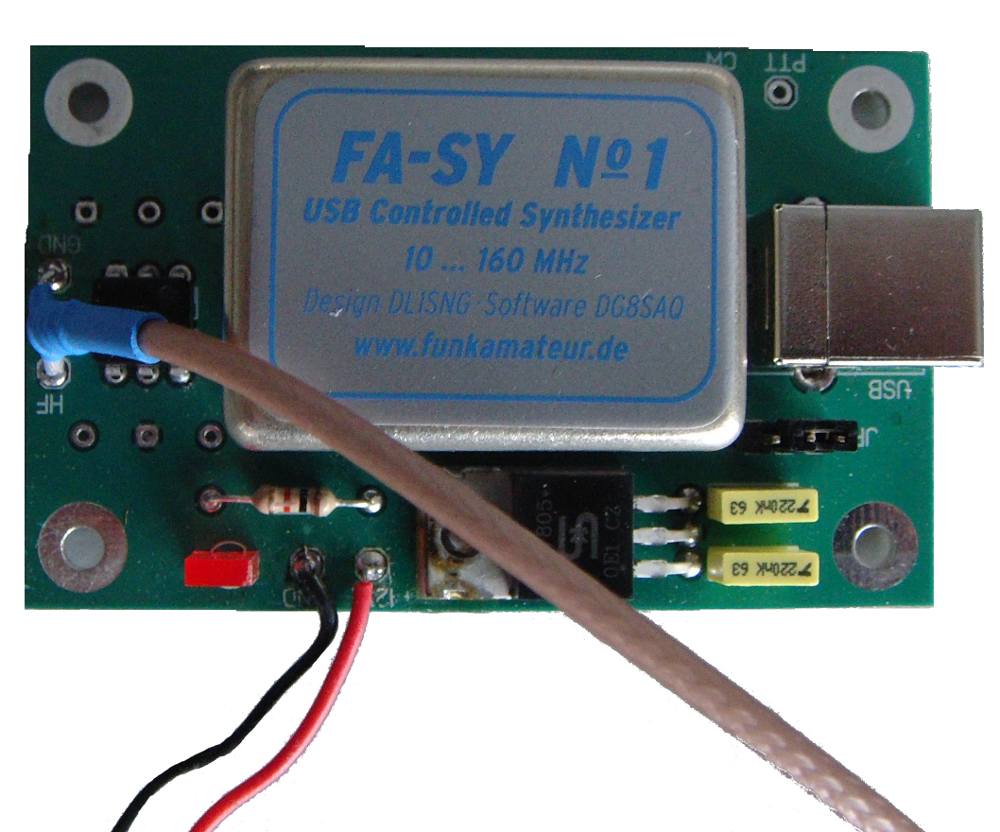
\includegraphics[width=0.50\textwidth]{img/frequenzgen.png}
    \caption{FA-Synthesizer}
	\label{fig:fasyn}
  \end{minipage}
\end{figure}
\end{itemize}
\begin{itemize}
\item \textbf{Asterisk}\\
OpenBTS benutzt eine herkömmliche PBX um die Gesprächsvermittlung zu realisieren und damit das klassische Mobile Switching Center (MSC) zu ersetzen. Wir setzen dabei die freie Software namens Asterisk ein die in OpenBTS unterstützt wird und neben der Hauptaufgabe, der Gesprächsvermittlung, weitere Features wie beispielsweise Mailbox-Services enthält. 
\end{itemize}
\begin{itemize}
\item \textbf{Smqueue}\\
Smqueue ist für den Versand bzw. die Speicherung von SMS Nachrichten zuständig. Darüber hinaus verfügt es über "`Short Code"'-Funktionalität, die es erlaubt den Inhalt von Textnachrichten als Eingabeargumente für selbst entwickelte lokale Anwendungen zu benutzen oder an eine E-Mail-Adresse weiterzuleiten.
Smqueue hat bereits eine solche Short-Code-Anwendung namens "`register"' integriert. Hierbei handelt es sich um eine interaktive Registrierung, bei der der Benutzer eine SMS mit der gewünschten Rufnummer als Inhalt an die BTS sendet. Wird diese Nummer noch nicht verwendet, trägt "`register"' diese zusammen mit der IMSI in die Subscriber Registry ein. %\footnote{Die interaktive Registrierung wurde von uns nicht getestet.}
\end{itemize}
\begin{itemize}
\item \textbf{Subscriber Registry}\\
Die Subscriber Registry ist eine Datenbank die OpenBTS für die Subscriber Informationen nutzt. Sie ersetzt zum einen das klassische GSM Home Location Register (HLR) und zum anderen die SIP Registry von Asterisk.
\end{itemize}

\textit{(Die Komponenten Smqueue und Subscriber Registry (sipauthserve) sind keine eigenständigen Projekte, sondern Bestandteile von OpenBTS.)}\\

In Abbildung \ref{fig:openbts_comp} sind die Beziehungen, sowie die Verbindungsprotokolle der einzelnen Komponenten untereinander ersichtlich.
\newpage
\begin{figure}[htbp]
	\centering
		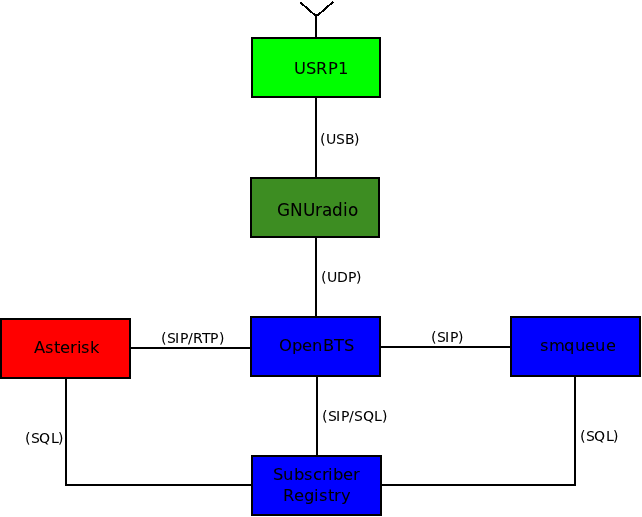
\includegraphics[width=0.80\textwidth]{img/openbts_comp.png}
	\caption{Systemkomponenten}
	\label{fig:openbts_comp}
\end{figure}


In Abbildung \ref{fig:openbts_system_diagram} ist noch einmal der Kommunikationsfluss im Hinblick auf SIP aufgezeichnet. Dabei kennzeichnen die \textbf{schwarzen} Pfeile SIP-Verbindungen, die \textcolor{red}{\textbf{roten}} Pfeile Datenbankabfragen und der \textcolor{blue}{\textbf{blaue}} Pfeil ODBC-Verbindungen.

\begin{figure}[hbtp]
	\centering
		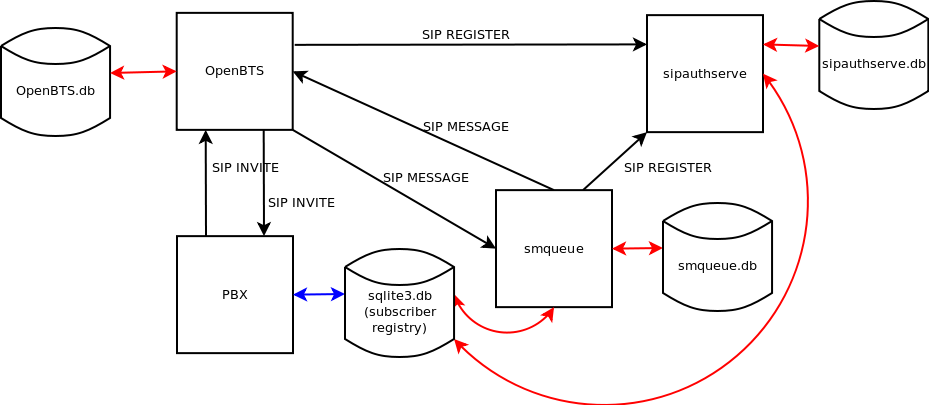
\includegraphics[width=1.00\textwidth]{img/openbts_system_diagram.png}
	\caption{System Diagramm (Quelle: \cite{bib:diagramm:openbts})}
	\label{fig:openbts_system_diagram}
\end{figure}
\subsubsection{Datenbanken}
Im System Diagramm findet man vier Datenbanken vor, welche für folgende Zwecke benutzt werden:

\begin{table}[h]
	\centering
		\begin{tabular}{ll}
			\textbf{OpenBTS.db} & Alle Konfigurationsparameter von OpenBTS werden\\
			& seit der Version P2.8 nicht mehr in einzelnen Konfi-\\
			& gurationsdateien hinterlegt, sondern in einer zentra-\\
			& len SQL-Datenbank verwaltet.\\
			\textbf{sipauthserve.db} & Hier werden die angemeldeten MS-Teilnehmer\\
			& registriert.\\
			\textbf{sqlite3.db} & Von Asterisk benutzte Datenbank zur SIP User\\ 
			& Registrierung, dessen Einträge von "`sipauthserve"'\\
			& erzeugt werden.\\
			 \textbf{smqueue.db} & Enthält alle Konfigurationsparameter von smqueue.\\
		\end{tabular}
\end{table}

\subsubsection{GSM/SIP-Abläufe}
\label{gsmsip} 
Einer der Hauptmerkmale von OpenBTS ist es, dass Mobile Switching Center (MSC) durch einen herkömmlichen VoIP-Switch (Asterisk) zu ersetzen. Dabei ist jede MS aus Sicht des Asterisk-Servers ein SIP-Endpunkt. Dieser SIP-Endpunkt wird von OpenBTS realisiert und verwaltet. Dabei wird jeder MS ein eigener SIP-Benutzername in der Form "`IMSIxxxxxxxxxxxxxxx"' zugeordnet, wobei die "`x"' der IMSI-Nummer der MS entsprechen. Die IP-Adresse jedes SIP-Endpunktes ist immer die gleiche und zwar die der BTS, also dort wo der OpenBTS-Dienst läuft. OpenBTS ist gegenüber Asterisk transparent, d.h. Asterisk sieht nur die MS als SIP-Endpunkte. Eine aktive Sprachverbindung besteht in diesem Kontext somit aus zwei Teilstrecken. Einmal die Strecke Asterisk $ \longleftrightarrow $ OpenBTS, in der SIP/RTP-Pakete die Sprachübertragung erledigen, und zum anderen die Strecke OpenBTS $ \longleftrightarrow $ MS, bei der ein GSM Sprach- bzw. Verkehrskanal (\textit{TCH}) auf der Luftschnittstelle existiert. Die SIP-Verbindung terminiert also bei OpenBTS.
\begin{figure}[h]
	\centering
		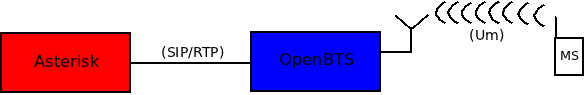
\includegraphics[width=0.80\textwidth]{img/openbts_sip_asterisk.png}
	\caption{Terminierung der SIP-Verbindung an OpenBTS}
	\label{fig:openbts_sip_asterisk}
\end{figure}

Die bereits oben erwähnte Komponente \textit{sipauthserve} ist dabei für die Registrierung der MS zuständig und trägt dazu  die Teilnehmer in die Datenbank \verb|sqlite3.db| ein.\\ 
Nachfolgend werden drei wesentliche GSM-Szenarien beschrieben, um das Zusammenspiel aus GSM- und SIP, wie in Abbildung \ref{fig:openbts_system_diagram} gezeigt, zu verdeutlichen:
\begin{itemize}
\item \textbf{Registrierung (Location Update)}\\
Wenn die MS eingeschaltet wird oder eine neue Location Area betritt, führt sie einen \textit{LOCATION UPDATE REQUEST} (LUR) aus. Zudem ist es möglich das die BTS die MS periodisch dazu auffordert ein LUR auszuführen. Bei OpenBTS wird ein GSM LUR in Form eines \textit{SIP REGISTER} durchgeführt (siehe Abb. \ref{fig:openbts_registration}). Zuerst findet der allgemeine GSM Ablauf der Kanalanforderung (ausgehend von der MS) statt. Nun folgt das eigentliche Location Update. Dazu schickt die MS einen \textit{LOCATION UPDATE REQUEST} an OpenBTS, welche daraufhin ein \textit{SIP REGISTER} an \textit{sipauthserve} sendet. \textit{sipauthserve} erstellt nun einen entsprechenden Eintrag in der SQL-DB \verb|sqlite3.db| (siehe Abb. \ref{fig:openbts_system_diagram}). Zum Schluss wird der zugewiesene GSM Kanal wieder abgebaut. Von nun an ist die MS im Netz registriert und kann durch einen \textit{PAGING REQUEST} "`angesprochen"' werden.
\begin{figure}[h]
	\centering
		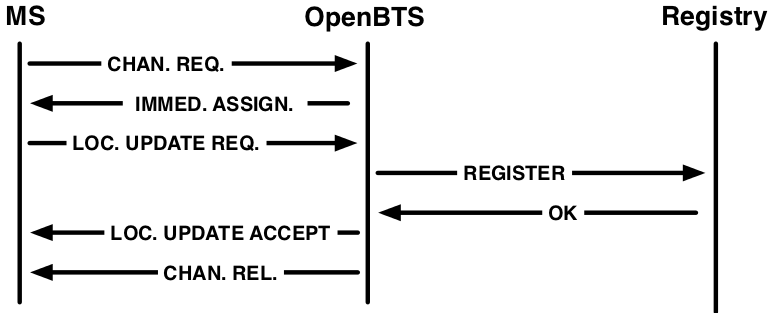
\includegraphics[width=0.80\textwidth]{img/openbts_registration.png}
	\caption{Location Update in Form eines SIP REGISTER (Quelle: \cite{bib:openbtsmanual}(S.47))}
	\label{fig:openbts_registration}
\end{figure}
\end{itemize}
\begin{itemize}
\item \textbf{Gesprächsaufbau (MS $\rightarrow$ SIP-Switch)}\\
Der Gesprächsaufbau ausgehend von der Mobile Station ist in Abbildung \ref{fig:openbts_call_msside} beschrieben. Die MS beantragt als erstes einen Kanal bei der BTS (\textit{CHANNEL REQUEST} auf \textit{RACH}), die BTS weist der MS daraufhin einen freien Kanal zu (\textit{IMMEDIATE ASSIGNMENT}), woraufhin dann diese eine Anfrage zum Verbindungsaufbau (\textit{CM SERVICE REQUEST}) an die BTS sendet. Akzeptiert die BTS die Anforderung, so folgt nun der eigentliche Aufbau des Gesprächs (\textit{SETUP}). OpenBTS sendet dazu einerseits einen \textit{SIP INVITE} an die PBX um eine SIP Session aufzubauen, und andererseits ein \textit{CALL PROCEEDING} zur Signalisierung an die MS. Wenn die SIP-Gegenstelle erreichbar ist (\textit{Status: 200 OK}) bekommt die MS dies als Läutezeichen (\textit{ALERTING}) mitgeteilt. Nimmt zudem die Gegenstelle das Gespräch an, so ist der Verbindungsaufbau komplett. Zwischen OpenBTS und PBX besteht nun eine RTP-Verbindung über die die Sprachpakete transportiert werden, und zwischen OpenBTS und MS besteht eine herkömmliche Sprachverbindung (\textit{TCH}) auf der GSM Luftschnittstelle.
\begin{figure}[h]
	\centering
		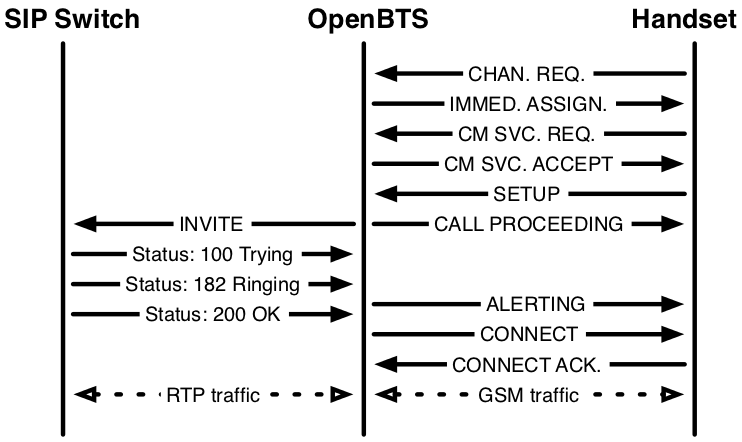
\includegraphics[width=0.80\textwidth]{img/openbts_call_msside.png}
	\caption{Gespräch ausgehend von der Mobile Station (Quelle: \cite{bib:openbtsmanual}(S.48))}
	\label{fig:openbts_call_msside}
\end{figure}
\end{itemize}
\begin{itemize}
\item \textbf{Gesprächsaufbau (SIP-Switch $\rightarrow$ MS)}\\
Zur Vollständigkeit sei in Abbildung \ref{fig:openbts_call_carrierside} der Gesprächsaufbau ausgehend vom SIP-Switch erwähnt. Diesmal kommt der \textit{SIP INVITE} von der PBX aus. OpenBTS versucht nun die MS zu erreichen (\textit{PAGING REQUEST}). Bei Erfolg fordert die MS wiederum einen Kanal bei der BTS an (siehe Punkt vorher), dass GSM Gespräch wird aufgebaut (\textit{SETUP}) und falls der MS-Benutzer nun endgültig das Gespräch annimmt, ist der Verbindungsaufbau komplett. Nun besteht wieder eine RTP-Verbindung zwischen PBX und OpenBTS, und eine Sprachverbindung (\textit{TCH}) auf der GSM Luftschnittstelle zwischen OpenBTS und MS. 
\begin{figure}[h]
	\centering
		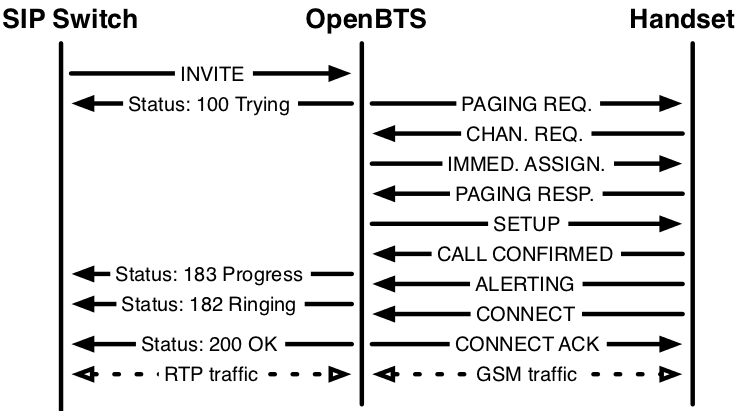
\includegraphics[width=0.80\textwidth]{img/openbts_call_carrierside.png}
	\caption{Gespräch ausgehend vom SIP-Carrier (Quelle: \cite{bib:openbtsmanual}(S.48))}
	\label{fig:openbts_call_carrierside}
\end{figure}
\end{itemize}

\subsection{Installation}
\label{sec:Installation}
Die Installation von \textbf{GNUradio, OpenBTS samt smqueue und sipauthserve}, sowie \textbf{Asterisk} erfolgte auf einem Ubuntu Linux 10.04.2 LTS. Dabei wurden die folgende Schritte bei der Installation des jeweiligen Softwarepakets durchgeführt.\\

\begin{center}
\begin{tabular}{l|l}
\textbf{Paket} & \textbf{Version}\\
\hline 
GNUradio & 3.4.2\\
OpenBTS & P2.8 (SVN)\\
smqueue & P2.8 (SVN)\\
sipauthserve & P2.8 (SVN)\\
Asterisk & 1.6.2.9 (Ubuntu Repository)\\
\end{tabular}
\end{center}
\textit{Auf Paketabhängigkeiten wurde größtenteils Rücksicht genommen. Sollte es trotzdem zu ungelösten Abhängigkeiten kommen, so können fehlende Pakete bspw. mittels} \verb|apt-get| \textit{aus entsprechenden Distributions-Repositories nachinstalliert werden.}

\subsubsection{GNUradio}
\textbf{GNUradio} wurde mit USRP1-Unterstützung kompiliert und installiert. 

\begin{enumerate}
	\item Fehlende Abhängigkeiten installieren:
	\begin{verbatim}
	sudo apt-get -y install git-core autoconf automake \
	libtool g++ python-dev swig pkg-config \
	libboost-all-dev libfftw3-dev libcppunit-dev \
	libgsl0-dev libusb-dev sdcc libsdl1.2-dev \
	python-wxgtk2.8 python-numpy python-cheetah \
	python-lxml doxygen python-qt4 python-qwt5-qt4 \
	libxi-dev libqt4-opengl-dev libqwt5-qt4-dev \
	libfontconfig1-dev libxrender-dev
	\end{verbatim}
	\item GNUradio mit USRP1-Unterstützung kompilieren und installieren:
	\begin{verbatim}
	wget http://gnuradio.org/redmine/attachments/\
	download/279/gnuradio-3.4.2.tar.gz
	tar xzf gnuradio-3.4.2.tar.gz
	cd gnuradio-3.4.2/
	./configure -with-usrp1
	make
	make check
	sudo make install
	\end{verbatim}
	\item Cache des Runtime Linkers aktualisieren:
	\begin{verbatim}
	export LD_LIBRARY_PATH=/usr/local/lib
	sudo ldconfig	
	\end{verbatim}
\end{enumerate}
 
\subsubsection{OpenBTS}
Für die Installation von \textbf{OpenBTS, smqueue und sipauthserve} wurde die aktuellste Version aus dem SVN-Repository verwendet.

\begin{enumerate}
	\item Fehlende Abhängigkeiten installieren:
	\begin{verbatim}
	sudo apt-get install autoconf libtool libosip2-dev \
	libortp-dev libusb-1.0-0-dev g++ sqlite3 \
	libsqlite3-dev erlang
	\end{verbatim}
	\item Sourcecode aus SVN-Repository kopieren:
	\begin{verbatim}
	mkdir openbts
	cd openbts
	svn co http://wush.net/svn/range/software/public
	\end{verbatim}
	\item In OpenBTS-Source-Verzeichnis wechseln und OpenBTS mit USRP1-Unterstützung kompilieren:
	\begin{verbatim}
	autoreconf -i
	./configure --with-usrp1
	make
	\end{verbatim}
	\item Da wir die USRP1 mit einem 52MHz Takt betreiben muss ein Link zur entsprechenden Transceiver-Binary erstellt, sowie die passende "`inband"'-Tabelle kopiert werden:
	\begin{verbatim}
	(from OpenBTS root)
	cd apps/
	ln -s ../Transceiver52M/transceiver .
	sudo mkdir -p /usr/local/share/usrp/rev4/
	sudo cp ../Transceiver52M/std_inband.rbf \
	/usr/local/share/usrp/rev4/
	cd ..
	\end{verbatim}
	\item Seit Version 2.8 wird die Konfiguration von OpenBTS nun nicht mehr in einzelnen großen Konfigurationsdatei gespeichert, sondern in einer SQL-Datenbank verwaltet. Diese erzeugen wir mit Hilfe des bereitgestellten Templates :
	\begin{verbatim}
	(from the OpenBTS directory)
	sudo mkdir /etc/OpenBTS
	sudo sqlite3 -init ./apps/OpenBTS.example.sql \
	/etc/OpenBTS/OpenBTS.db
	( .exit zum verlassen von sqlite3)
	\end{verbatim}
\end{enumerate}

\subsubsection{Subscriber Registry und Sipauthserve}
\begin{enumerate}
	\item Zuerst sollte \textbf{Asterisk} installiert werden damit die entsprechenden Verzeichnisse existieren:
	\begin{verbatim}
	sudo apt-get install asterisk
	\end{verbatim}
	\item Im SVN-Repository befindet sich ein SQL-Skript das nun für die Erstellung der Subscriber Registry benutzt wird:
	\begin{verbatim}
	(from svn root)
	cd public/subscriberRegistry/trunk/configFiles/
	sudo mkdir /var/lib/asterisk/sqlite3dir
	sudo sqlite3 -init subscriberRegistryInit.sql \
	/var/lib/asterisk/sqlite3dir/sqlite3.db
	( .exit zum verlassen von sqlite3)
	\end{verbatim}
	\item Nun wird \textbf{sipauthserve} kompiliert und dessen Konfigurationsdatenbank in \verb|/etc/OpenBTS/| erzeugt:
	\begin{verbatim}
	(from svn root)
	cd subscriberRegistry/trunk
	make
	sudo sqlite3 -init sipauthserve.example.sql \
	/etc/OpenBTS/sipauthserve.db
	( .exit zum verlassen von sqlite3)
	\end{verbatim}
\end{enumerate}

\subsubsection{Smqueue}
\begin{enumerate}
	\item \textbf{Smqueue} kompilieren:
	\begin{verbatim}
	(from svn root)
	cd smqueue/trunk/
	autoreconf -i
	./configure
	make
	\end{verbatim}
	\item Konfigurationsdatenbank von smqueue in \verb|/etc/OpenBTS/| erzeugen
	\begin{verbatim}
	sudo sqlite3 -init smqueue/smqueue.example.sql \
	/etc/OpenBTS/smqueue.db
	( .exit zum verlassen von sqlite3)
  \end{verbatim} 
\end{enumerate}

\subsection{Konfiguration}
\label{sec:Konfiguration}
\subsubsection{OpenBTS}
Die Datenbank \verb|/etc/OpenBTS/OpenBTS.db| enthält sämtliche Konfigurationsparameter für OpenBTS. Eine Liste aller Parameter, sowie dessen Beschreibung, findet man unter \url{https://wush.net/trac/rangepublic/wiki/openBTSConfig}.
Die Parameter können entweder direkt in der Datenbank \verb|OpenBTS.db| (z.B. mittels \verb|sqlite3 /etc/OpenBTS/OpenBTS.db|) oder am OpenBTS-Prompt mit den Befehlen \verb|config| bzw. \verb|unconfig| geändert werden.

Für die meisten Parameter eignen sich die bereits eingetragenen Standardwerte, jedoch sind einige grundlegende Einstellungen vorzunehmen:

\begin{itemize}
  \item \textbf{GSM.Radio.Band}\\
  Bestimmt das benutzte GSM-Band, bei uns: \textbf{1800}
  \item \textbf{GSM.Radio.C0}\\
  Die ARFCN Nummer, bei uns: \textbf{867}
  \item \textbf{GSM.CellSelection.Neighbors}\\
  ARFCN der Nachbarzellen, bei uns: \textbf{846}
  \item \textbf{Control.LUR.OpenRegistration}\\
  Mittels eines regulären Ausdrucks werden die IMSIs definiert, die sich an der BTS registrieren dürfen. Für Testzwecke ist es jedoch sinnvoll eine offene Registrierung zu verwenden, d.h. es darf sich jede MS verbinden. Dazu ist der Wert auf \textbf{Null} zu setzen.
  \item \textbf{GSM.Identity.MCC}\\
  Der Mobile Country Code bestimmt ist die Länderkennung, bei uns: \textbf{262} für Deutschland.
  \item \textbf{GSM.Identity.MNC}\\
  Der Mobile Network Code ist eine zweistellige Nummer die den Mobilfunkanbieter kennzeichnet. In Deutschland besitzt T-Mobile beispielsweise die 01, E-Plus die 03 und O2 die 07. Wir haben den Wert \textbf{99} eingestellt, da sich dieser offiziell nicht in Gebrauch befindet.
  \item \textbf{GSM.Identity.ShortName}\\
  Kurze Bezeichnung des Netzwerks; wird bei manchen Mobilfunktelefonen im Display angezeigt (überwiegend neuere Modelle); bei uns \textbf{OpenBTS HM}
  \item \textbf{GSM.RACH.AC}\\
  Die Access Class Flags sollten bei einem nicht funktionstüchtigen Netz auf \verb|0x0400| gesetzt werden, um dem Benutzer mitzuteilen, dass keine Notrufunterstützung existiert.    
\end{itemize} 

\subsubsection{Sipauthserve}
In der Regel müssen keine weiteren Einstellungen vorgenommen werden, solang man den Standardpfad für die \verb|sqlite3.db| eingehalten hat. Hat man dies nicht, so ist der neue Dateipfad (Feld: \verb|SubscriberRegistry.db|) in der Konfigurationsdatenbank (\verb|/etc/OpenBTS/sipauthserve.db|) anzugeben. Hilfreich könnte auch das Hochsetzen des \verb|Log.Level| sein, welches standardmäßig auf \textit{WARNING} eingestellt ist und unter \textit{DEBUG} deutlich mehr Hinweise bzgl. der erstellten Registry-Einträge offenbart.

\subsubsection{Smqueue}
Auch an der Konfiguration von \textit{smqueue} muss zwangsläufig keine Änderung vorgenommen werden. Allerdings enthält die Konfigurationsdatenbank (\verb|/etc/OpenBTS/smqueue.db|) weitaus mehr Einträge als die von sipauthserve. Gut die Hälfte dieser Parameter beziehen sich auf die "`Short Code"'-Funktionalität.

\subsubsection{Asterisk}
Die Konfiguration von Asterisk beschränkt sich in diesem Dokument auf die Intra-BTS-Kommunikation, d.h. es können nur Gespräche zwischen MS und MS bzw. MS und Asterisk-Diensten (Echo-Test, VoiceMail) statt finden, nicht jedoch von oder nach Außerhalb (Festnetz, andere SIP-Teilnehmer) telefoniert werden.
\begin{itemize}
\item \textbf{Teilnehmereintrag}\\\label{asterisk_teilnehmer}Damit die MS untereinander telefonieren können, müssen die Asterisk-Konfigurationsdateien \verb|sip.conf| und \verb|extensions.conf| im Verzeichnis \verb|/etc/asterisk/| angepasst werden. Als Beispiel wird die \textbf{IMSI 001010000000000} verwendet und dieser die Teilnehmerrufnummer \textbf{2101} zugeordnet.\\

In \verb|sip.conf| muss folgender Eintrag hinzugefügt werden:
\newpage
\begin{figure}[ht]
\setbox0\vbox{\small
\begin{verbatim}

...
[IMSI001010000000000]
callerid=2101         ; Teilnehmerrufnummer (diese
                      ; sieht auch die Gegenstelle)
canreinvite=no        ; Asterisk ist Mittelsmann
                      ; zwischen MS und Gegenstelle
type=friend           ; MS ruft uns bzw. wir rufen MS an
context=sip-external  ; zugeordneter Kontext
allow=gsm             ; Sprachcodec 'gsm' erlauben
host=dynamic          ; dynamischer Hostname
dtmfmode=rfc2833      ; DTMF-Töne nach Standard RFC2833
...
\end{verbatim}
}
\centerline{\fbox{\box0}}
\end{figure}

In \verb|extensions.conf| muss je IMSI ein Eintrag in der ihr zugeordneten Extension (hier \verb|sip-external|) hinzugefügt werden:
\begin{figure}[ht]
\setbox0\vbox{\small
\begin{verbatim}

...
[sip-external]
exten => 2101,1,Dial(SIP/IMSI001010000000000@127.0.0.1:5062)
...
\end{verbatim}
}
\centerline{\fbox{\box0}}
\end{figure}
\end{itemize}
\begin{itemize}
\item \textbf{Echo-Test}\\Zu Testzwecken empfiehlt es sich einen sog. "`Echo-Test"' unter Asterisk zu konfigurieren. Bei einem Echo-Test wird alles was man sagt als Echo zurückgeschickt. Zum einen erkennt man dadurch welche Latenzzeit zwischen MS und Asterisk besteht und zum anderen lässt sich ein Sprachkanal ohne die Notwendigkeit einer zweiten MS einfach aufbauen.
Um den Echo-Test zu aktivieren, werden folgende Zeilen in die \verb|extensions.conf| innerhalb des Kontext \verb|[sip-external]| eingefügt:
\begin{figure}[ht]
\setbox0\vbox{\small
\begin{verbatim}

[sip-external]
...
exten => 600,1,Answer()
exten => 600,2,Playback(demo-echotest)
exten => 600,3,Echo()
exten => 600,4,Playback(demo-echodone)
exten => 600,5,Hangup()
...
\end{verbatim}
}
\centerline{\fbox{\box0}}
\end{figure}

Nun ist der Echo-Test unter der Rufnummer 600 zu erreichen.\\

In der Praxis zeigte sich, dass die Sprachverzögerung um die 0.5 Sekunden liegt, was mit hoher Wahrscheinlichkeit an OpenBTS liegt. Ein zweiter Test zwischen Asterisk und einem herkömmlichen SIP-Client (Software), über eine direkte VoIP-Verbindung, wies nämlich keine nennenswerte Latenz auf.
\end{itemize}
\begin{itemize}
\item \textbf{VoiceMail}\\Jedem eingetragenen Teilnehmer kann eine Mailbox zugeordnet werden, welche aktiv wird wenn der Teilnehmer entweder nicht erreichbar ist (im Netz nicht registriert) oder nach einer einstellbaren Zeit den Anruf nicht entgegennimmt.
Für die Einrichtung einer Mailbox sind die folgende Schritte notwendig:
\begin{enumerate}
\item Neuen Kontext und Benutzer in \verb|/etc/asterisk/voicemail.conf| hinzufügen:
\begin{figure}[ht]
\setbox0\vbox{\small
\begin{verbatim}

...
[mailbox]
2101 => 1234, 2101		; #Rufnummer => #Passwort, #Benutzer
;weitere VoiceMail-Benutzer
...
\end{verbatim}
}
\centerline{\fbox{\box0}}
\end{figure}
\item Regelwerk in \verb|/etc/asterisk/extensions.conf| anpassen und VoiceMail-Abfrage hinzufügen:
\begin{figure}[ht]
\setbox0\vbox{\small
\begin{verbatim}

...
[sip-external]
exten => 2101,1,Dial(SIP/IMSI001010000000000
         @127.0.0.1:5062,20)
exten => 2101,2,VoiceMail(2101@mailbox)
exten => 2101,3,PlayBack(vm-goodbye)
exten => 2101,4,HangUp()

exten => 8888,1,VoiceMailMain(s${CALLERID(num)}@mailbox)	; Abfrage ohne Auth.
exten => 9999,1,VoiceMailMain(@mailbox)						; Abfrage mit Auth.
...
\end{verbatim}
}
\centerline{\fbox{\box0}}
\end{figure}

Das obige Regelwerk des Benutzers mit der Teilnehmerrufnummer 2101 besagt folgendes:\\
Zuerst wird versucht den Benutzer \textbf{IMSI001010000000000} über SIP zu erreichen (siehe Kapitel \ref{gsmsip}). Falls er im Netz registriert ist und die MS über \textit{PAGING} erreichbar ist, wird man nun maximal 20 Sekunden lang anläuten und nach Ablauf dieser Zeit zu Regel 2 springen. Ist der Benutzer erst gar nicht im Netz registriert, so wird unmittelbar zu Regel 2 gesprungen. Regel 2 definiert den eigentlichen Mailbox-Befehl. Der Anrufende hört die Mailboxansage und hat die Möglichkeit eine Nachricht zu hinterlassen. Hat er dies getan, so kann er entweder direkt auflegen oder mittels der Rautetaste die Aufnahme beenden. Regel 3 spielt daraufhin ein "`Auf wiedersehen"'-Soundfile ab und Regel 4 beendet letztendlich den Anruf.

Zur Mailbox-Abfrage hat man zwei Möglichkeiten. Ruft man, in unserem Beispiel, die Nummer \textbf{8888} an, so gelangt man direkt, d.h. ohne interaktive Authentifizierung, zu seinem Mailbox-Menü. Dort kann man aufgenommene Nachrichten abspielen, verwalten, löschen und weitere Mailbox-Optionen treffen. Unter der \textbf{9999} muss man sich erst mit seiner Mailbox-Kennung (hier im Beispiel ist das die 2101) und seinem Passwort (1234) gegenüber der Mailbox-Abfrage authentifizieren.

In der Praxis kam es zu Problemen bei der interaktiven Mailbox-Abfrage. Die Kennung und/oder das Passwort wurden als falsch von Asterisk betrachtet und eine erfolgreiche Authentifizierung war nicht möglich. Der Grund hierfür dürfte an einem nicht unterstützten bzw. nicht konfigurierten DTMF-Modus liegen, mittels dem die Tasteneingabe (Tastentöne) übertragen werden. Aus Zeitgründen und weil die Mailbox-Abfrage für unser Projektziel nicht relevant war, wurde der Sache nicht weiter auf den Grund gegangen.
\end{enumerate}
\end{itemize} 

\subsection{Benutzung von OpenBTS}
\subsubsection{Start der Dienste}
Damit die Registrierung der Teilnehmer und der Versand von Textnachrichten möglich ist, müssen neben OpenBTS auch die beiden Dienste \verb|sipauthserve| sowie \verb|smqueue| gestartet werden.
\begin{verbatim}
(from svn root)
./smqueue/trunk/smqueue/smqueue &
./subscriberRegistry/trunk/sipauthserve &
./openbts/trunk/apps/OpenBTS
\end{verbatim}

\subsubsection{Registrierung einer MS an OpenBTS}
Mit Hilfe der bereitgestellten Mobiltelefone vom Typ "`Nokia 3330"' und der programmierbaren SIM-Karten von Giesecke \& Devrient konnte nun eine Registrierung in unserem GSM Testnetz namens "`OpenBTS HM"' stattfinden. Dank der offenen Registrierung (\verb|Control.LUR.OpenRegistration|) kann man sich einfach am Netz registrieren und erhält zudem eine SMS, dessen Inhalt über den Konfigurationsparameter \verb|Control.LUR.OpenRegistration.Message| bestimmbar ist. Wichtiger Bestandteil dieser Kurzmitteilung ist die IMSI der SIM-Karte mit der sich die MS an der BTS registriert hat. Nun kann ein Teilnehmereintrag in Asterisk, wie in Kapitel \ref{asterisk_teilnehmer} beschrieben, erfolgen.\\
Folgendes Beispiel zeigt den SMS-Inhalt für die IMSI 262071111111111:
\begin{figure}[ht]
\setbox0\vbox{\small
\begin{verbatim}
Welcome to the GSM test network. Your IMSI is
IMSI:262071111111111
\end{verbatim}
}\centerline{\fbox{\box0}
}
\end{figure}

\subsubsection{Command Line Interface (CLI)}
Konnte OpenBTS erfolgreich gestartet werden, sieht man nun das Command Line Interface (CLI) vor sich:
\begin{figure}[ht]
\setbox0\vbox{\small
\begin{verbatim}
OpenBTS>
\end{verbatim}
}\centerline{\fbox{\box0}
}
\end{figure}\\
Nachfolgend einige Beispiele von hilfreichen CLI-Befehlen:
\begin{itemize}
\item \textbf{Befehl:} \verb|calls|\\
Listet aktive Gesprächs- bzw. SMS-Aktivitäten auf.
\begin{figure}[ht]
\setbox0\vbox{\small
\begin{verbatim}
OpenBTS> calls
2060207953 C0T1 TCH/F IMSI=001010000000000 L3TI=8 
SIP-call-id=1811340387 SIP-proxy=127.0.0.1:5060 MOC
to=600 GSMState=active SIPState=Active (5 sec)
\end{verbatim}
}\centerline{\fbox{\box0}
}
\end{figure}\\
Dabei ist \verb|2060207953| die Transaktions-ID, \verb|C0T1| die C0-ARFCN und der dabei verwendete Zeitschlitz (\textit{Nr. 1}), \verb|TCH/F| die Kanalart (\textit{Full-Rate Traffic Channel}) und \verb|IMSI=001010000000000| die IMSI des Teilnehmers. Die restlichen Angaben beziehen sich auf die SIP-Verbindung (\textit{ID, SIP-Status und Verbindungsdauer}).
\end{itemize}
\newpage
\begin{itemize}
\item \textbf{Befehl:} \verb|chans|\\
Listet aktive Kanäle und die dazugehörigen Leistungswerte auf.
\begin{figure}[ht]
\setbox0\vbox{\small
\begin{verbatim}
OpenBTS> chans
CN TN chan     transaction UPFER RSSI TXPWR TXTA DNLEV DNBER
CN TN type     id          pct    dB   dBm  sym   dBm   pct
 0 1    TCH/F  1247828231  0.54  -53    30    1   -48  0.00
\end{verbatim}
}\centerline{\fbox{\box0}
}
\end{figure}\\
Im obigen Beispiel handelt es sich um einen Verkehrskanal im Full-Rate Modus (\verb|TCH/F|) der den ersten Zeitschlitz (\verb|TN=1|) belegt und der Transaktions-ID \verb|1247828231| zugeordnet ist. Die MS sendet mit \verb|30 dBm| (\verb|TXPWR|) und besitzt einen Timing Advance (\verb|TXTA|) Wert von \verb|1|. Die beiden Angaben \verb|UPFER| und \verb|RSSI| beziehen sich auf den Uplink. \verb|UPFER| gibt dabei die Fehlerrate der Frames an, die im Beispiel bei \verb|0,54| Prozent liegt, und \verb|RSSI| die Stärke des Sendesignals der MS, hier \verb|-53 dBm|. Für den Downlink gibt \verb|DNBER| die Fehlerrate der Bits an und \verb|DNLEV|, dass Pendant zu RSSI im Uplink, gibt die Empfangssignalstärke der MS, hier \verb|-48 dBm|, an.
\end{itemize}
\begin{itemize}
\item \textbf{Befehl:} \verb|tmsis|\\
Listet die aktuelle TMSI-Tabelle auf.
\begin{figure}[ht]
\setbox0\vbox{\small
\begin{verbatim}
OpenBTS> tmsis
TMSI       IMSI             age   used
1          001010000000000  138s  138s
\end{verbatim}
}\centerline{\fbox{\box0}
}
\end{figure}\\
Im Beispiel wurde der IMSI \verb|001010000000000| die TMSI \verb|1| zugeordnet. Dieser Eintrag wurde vor 138s (\verb|age|) erstellt. Ebenfalls 138s ist diese TMSI in Gebrauch (\verb|used|). 
\end{itemize}

Eine Liste aller möglichen OpenBTS-Befehle sowie dessen Beschreibung findet sich unter \url{https://wush.net/trac/rangepublic/wiki/cli} oder im Benutzerhandbuch von OpenBTS \cite{bib:openbtsmanual}(Kapitel 5.5).


